    We are building an implementation of CLINT to debug SDN networks running the POX network operating system~\cite{pox}.
    
    POX is an implementation of the NOX network operating system built in Python.
    POX applications are typically written for a single controller with only minimal virtualization.
    To study \projectname{}'s ability to capture virtualization errors, we extended POX
    to support a simple virtualization layer that presents switches as Python objects to the control application.
    The virtualization layer does not yet support more complex virtualization such as `big switch' representations 
    of the network; in future work we plan to extend it to so.
    To study bugs that arise between replicated controllers, we also extended POX to support replicated controllers
    with eventually-consistent shared state.

    The current implementation of CLINT supports two features outlined in \S\ref{sec:architecture}, a traffic and topology `fuzzer' for input generation, and an invariant checker to detect bugs that manifest in the physical network.
    Our invariant checker is an extension of the Anteater~\cite{anteater} network debugger.
    In future work, we plan to develop a correspondence checker to do cross-layer and cross-controller analysis.

    We evaluated the existing features of \projectname{} by testing it to check for invariant violations in the physical network (\S\ref{sec:invariantdetection}), using the fuzzer to detect errors that manifest depending on the order of flows and configuration of the network topology (\S\ref{sec:fuzztest}), and by stress-testing \projectname{} against large topologies to quantify the overhead imposed by running \projectname{} in iteration over large topologies (\S\ref{sec:overhead}). 
    \subsection{Invariant Detection}

    \subsection{Fuzzing}

        
    \subsection{System Overhead}

    There is already a nice evaluation of Anteater. Something like 400 seconds for
    a large network.

    Now we're running Anteater in a
    loop. Is this going to take rediculously long? We hope not.

    \begin{figure}[t]
        \centering
        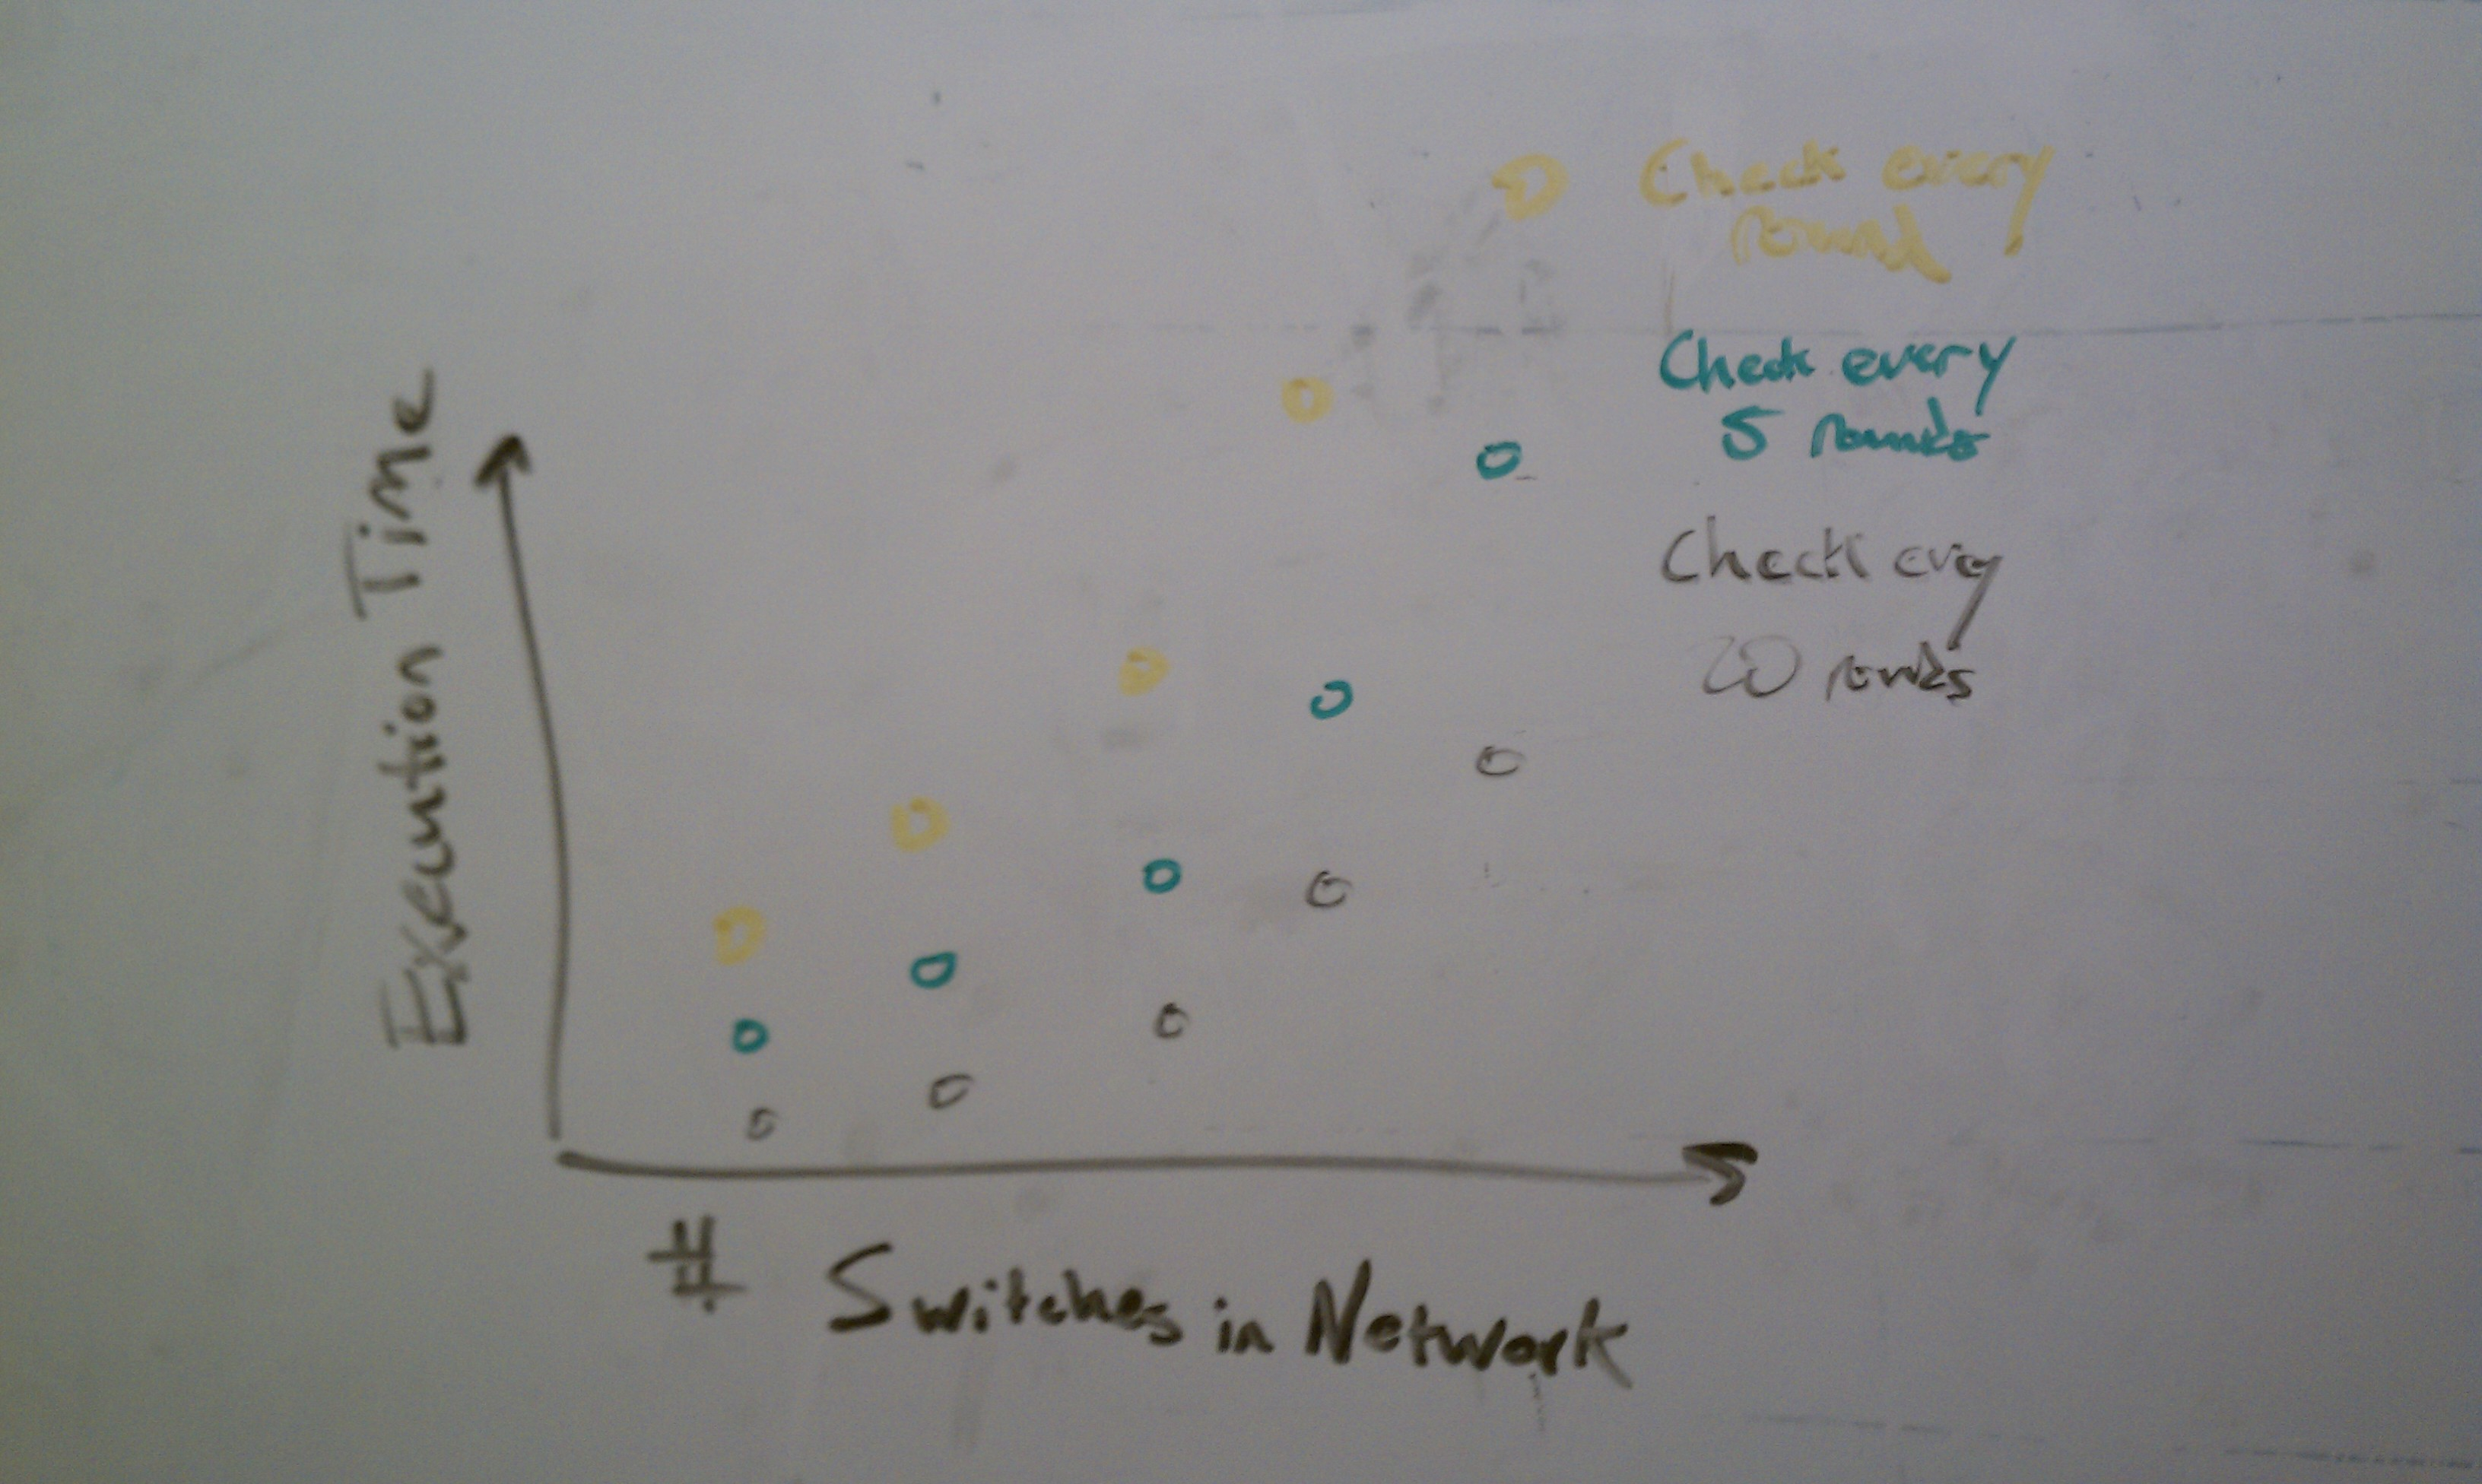
\includegraphics[width=3in]{../graphs/mock_overhead_graph.jpg}
        \caption[]{\label{fig:loop} Our lovely graph showing that execution time
        is not too bad\vspace{-10pt}} 
    \end{figure}

    Two orthogonal ways to ameliorate the overhead. First, you could intellegintly choose
    when to run Anteater, so that you don't have to run it for every possible
    configuration, while still getting good coverage of the
    configuration space. Second, you could make Anteater faster, perhaps by only
    getting `best-effort` exploration of the invariant checks rather than
    full-blown proofs that the invariant holds. Also, Brighten mentioned that the
    current version of Anteater runs significantly faster.

    \subsection{Next Steps}
        The previously described experiments show that our implementation of \projectname{} (1) can detect errors like forwarding loops that manifest entirely in the physical network (by using Anteater), (2) can detect physical network errors that manifest as the result of a specific sequence of flows to reach the network controller (by using \projectname{}'s network fuzzer), and (3) imposes reasonable performance requirements to analyze the SDN stack for these errors.
        To complete this analysis, we are working with engineers at Nicira Networks to obtain in-depth bug reports describing errors encountered by real SDN deployments.
        In future work, we plan to replicate these bugs in our SDN testbed and investigate whether \projectname{} can detect them.
        In addition, we are working with researchers at the International Computer Science Institute (ICSI) to obtain copies of their own SDN control applications from their research, and apply \projectname{} to their implementations to investigate whether \projectname{} can detect any new bugs.

        Longer term, as the \projectname{} implementation matures to include multi-layer correspondence checks and cross-controller consistency checks (as described in \S\ref{sec:architecture}), we will apply \projectname{} to a broader class of bugs and see what fraction of Nicira bug reports \projectname{} can capture, and what kinds of new bugs it detects in control applications from ICSI. 


